%!TEX root =conext14.tex
\section{Performance Evaluation}
\label{sec:evaluation}
To evaluate the performance of our proposed system, we implemented our multipath IP in Ubuntu under Linux kernel $3.12.1$. Two desktops are installed with the MPIP enabled Ubuntu system. At each desktop, two NICs working at $25$Mbits/sec are installed which means that there are totally $4$ paths and the throughput upper bound is $50$Mbits/sec between the two nodes. We modify an open source software \bf{Simple Traffic Monitor}\cite{simon01} to record the real time traffic that goes through each NIC.

%For mobile devices, we implement this feature in Google Nexus $4$ with Android $4.01$.

\subsection{TCP/UDP throughput enhancement}
\label{sec:tcp}

In this section, we try to verify that our system can achieve high throughput in both TCP and UDP scenarios. As a typical implementation of multipath, MPTCP creates the highest TCP throughput record between two nodes in \cite{record}. In that demonstration, they used $6$ $1$Gbps NIC interfaces at each node, and connect them directly without only middle boxes, and they limited the number of paths to $6$ by setting up IP TABLES in Ubuntu. Also, they did bunch of TCP parameter optimization to squeeze out all possible throughout. They achieved a breathtaking $51$Gbps throughput in that demonstration. 

We don't have the same configuration of the record-breaking plat of MPTCP, but we use the same typical configuration for all scenarios to do side-by-side configuration. We try to verify that our implementation can achieve the same throughput improvement as MPTCP for TCP traffic, and also our system can have the same enhancement for UDP traffic. 

In our experiment setup, we have two PCs while each PC has two NIC cards, every NIC card works at 100Mbps. With these four NIC cards, we have different configurations to verify our system. For each configuration, we do side-by-side comparision among regular connection, MPTCP(For TCP), and MPIP connection. We use iperf to transmit traffic for five minutes, and we customized iperf to record real-time throughput of each second.

In Figure~\ref{fig.nonat}, we connect the two machine to the same router which means there are no NAT devices on all the paths.

\begin{figure*}[htb]
\centering{
\subfigure[TCP throughput with psudo TCP connection\label{fig.tcp_usetcp_nonat}]{\includegraphics[width=0.33\linewidth]{fig/tcp_usetcp_nonat.eps}}
\subfigure[TCP throughput with UDP Wrapper\label{fig.tcp_useudp_nonat}]{\includegraphics[width=0.33\linewidth]{fig/tcp_useudp_nonat.eps}}
\subfigure[UDP throughput\label{fig.udp_nonat}]{\includegraphics[width=0.33\linewidth]{fig/udp_nonat.eps}}
}
\caption{Side-by-side comparison without NAT}
\label{fig.nonat}
\end{figure*}

Also, we set up a NAT network with two routers as shown in Figure~\ref{fig.nat}. Because our router only has 100Mbps capacity while each NIC has 100Mbps, this means that our router can't fit all capacity of the NIC cards. To avoid this problem, we limit the bandwidth of our NIC cards to be 5Mbps with WonderShaper. Then the total capacity of our connection is 10Mbps. Figure~\ref{fig.nat} shows the result for this configuration.

\begin{figure*}[htb]
\centering{
\subfigure[TCP throughput with psudo TCP connection\label{fig.tcp_usetcp_nat}]{\includegraphics[width=0.33\linewidth]{fig/tcp_usetcp_nat.eps}}
\subfigure[TCP throughput with UDP Wrapper\label{fig.tcp_useudp_nat}]{\includegraphics[width=0.33\linewidth]{fig/tcp_useudp_nat.eps}}
\subfigure[UDP throughput\label{fig.udp_nat}]{\includegraphics[width=0.33\linewidth]{fig/udp_nat.eps}}
}
\caption{Side-by-side comparison with a simple NAT}
\label{fig.nat}
\end{figure*}


In Figure~\ref{fig.net}, we set up our server in Emulab to verify our system in Internet. Because the server in Emulab only has one public IP address which means our connection only has two paths. Also, Emulab doesn't support iperf with UDP traffic, so we only test TCP scenario.

\begin{figure}[htb]
\centering{
\subfigure[TCP throughput with psudo TCP connection\label{fig.tcp_usetcp_net}]{\includegraphics[width=0.49\linewidth]{fig/tcp_usetcp_net.eps}}
\subfigure[TCP throughput with UDP Wrapper\label{fig.tcp_useudp_net}]{\includegraphics[width=0.49\linewidth]{fig/tcp_useudp_net.eps}}
}
\caption{Side-by-side comparison in Internet}
\label{fig.net}
\end{figure}


\subsection{Skype voice call improvement}
\label{sec:skype}

In Figure~\ref{fig.skype}, we prove that our packet-size based routing decision works perfectly for audio application like Skype. In our experiment, we change the delay of NIC cards using the netem package in Ubuntu. On one side of the Skype call, we have two NIC cards as stated above. We ran the experiment for $360$ seconds with $3$ sections. In the first $120$ seconds, there is no manually added delay on each NIC card, we add additional $120ms$ delay to the first NIC card in the following $120$ seconds, finally for the last $120$ seconds, we add $120ms$ delay to the second NIC card. We did our Skype audio experiment without video content while most packets on the connection are audio packets except some control packets.The size of Audio packets is relative small, generally under $200$KB. In this case, according to Equation~\ref{eq.bw} to Equation~\ref{eq.c}, the routing decision will mostly depend on the delay value instead of queuing delay. Figure~\ref{fig.skype} shows the packets routing adaptation as the delay value changes. By this adaptation, we can make sure that the audio streaming will always choose the path that has lower delay to keep the best user experience even other paths have the same throughput.

\begin{figure}
\centering
\includegraphics[width=1\linewidth]{fig/skype.eps}
\caption{Skype Audio Streaming Routing Adaptation}
\label{fig.skype}
\end{figure}


\subsection{Smooth connection switch}
\label{sec:switch}

In Figure~\ref{fig.switch}, we verify that smooth switch between different NIC cards works perfectly over our MPIP implementation by doing an IPERF TCP experiment. We do a side-by-side comparison between MPIP and MPTCP. We also divide the experiment into $3$ sections with $120$ seconds for each section. On the client side of the connection, there are two NIC cards. In the first $120$ seconds, both NIC cards work synchronously, then we disable one of them for $120$ seconds, and during the last $120$ seconds, we enable back the NIC card. The result shows that our MPIP system can follow this on/off process perfectly with stable throughput. For MPTCP, besides the fluctuating throughput which also happened in previous experiments, when trying to enable back the disabled NIC card, the throughput doesn't come back at all. According to monitoring the TCP connections between the client the server, MPTCP does constructs two new TCP connections after enabling back the NIC card, but it doesn't transmit any data after coming back.

\begin{figure}
\centering
\includegraphics[width=1\linewidth]{fig/switch.eps}
\caption{Connection Smooth Switch}
\label{fig.switch}
\end{figure}
%
%\subsection{Datacenter use case}
%\label{sec:datacenter}
%
%\subsection{Seamless handover with dynamic networks}
%\label{sec:handover}
